\documentclass{article}
\usepackage[utf8]{inputenc}
\usepackage{graphicx}
\graphicspath{ {images/} }
\usepackage{amsmath}
\usepackage{gensymb}
\usepackage[english]{babel}
\usepackage[version=4]{mhchem}
\usepackage[T1]{fontenc}
\usepackage{wrapfig}
\usepackage[colorlinks,allcolors = blue]{hyperref} 
%\numberwithin{equation}{section}
%\numberwithin{figure}{section}
%\numberwithin{table}{section}

%\usepackage[font=scriptsize,labelfont=bf]{caption}
%\usepackage{subcaption}
\usepackage[backend=biber,style=authoryear-comp]{biblatex}
\usepackage[a4paper, portrait, margin=1in]{geometry}
\addbibresource{mybib_stable.bib}
\usepackage{listings}
\usepackage{xcolor}

\definecolor{codegreen}{rgb}{0,0.6,0}
\definecolor{codegray}{rgb}{0.5,0.5,0.5}
\definecolor{codepurple}{rgb}{0.58,0,0.82}
\definecolor{backcolour}{rgb}{0.95,0.95,0.92}

\lstdefinestyle{mystyle}{
    backgroundcolor=\color{backcolour},   
    commentstyle=\color{codegreen},
    keywordstyle=\color{magenta},
    numberstyle=\tiny\color{codegray},
    stringstyle=\color{codepurple},
    basicstyle=\ttfamily\footnotesize,
    breakatwhitespace=false,         
    breaklines=true,                 
    captionpos=b,                    
    keepspaces=true,                 
    numbers=left,                    
    numbersep=5pt,                  
    showspaces=false,                
    showstringspaces=false,
    showtabs=false,                  
    tabsize=2
}

\lstset{style=mystyle}

\setlength{\parindent}{4em}
\setlength{\parskip}{1em}
\renewcommand{\baselinestretch}{1.5}

% \title{GIS For Dummies: Live Demonstration Guide}
% \author{Nicholas D. Barber}
% \date{\today}

\begin{document}

\begin{titlepage}
   \begin{center}
       \vspace*{1cm}

       \LARGE
       \textbf{GIS for Geoscientists: Live Demo Guide}
       
       \Large
       \vspace{0.3cm}
        Companion exercise guides for the GIS for Geoscientists Workshop Series. Originally prepared for McGill University in June of 2020. 
            
       \vspace{1.2cm}
       \textbf{Nicholas D. Barber}\\
       Department of Earth Science\\
       University of Cambridge\\
       United Kingdom\\
       \today
            
       \vspace{0.8cm}
     
       \includegraphics[width=0.9\textwidth]{Figure1_HazardMap_GP.png}
   \end{center}
\end{titlepage}

\tableofcontents

\section{Course Overview}

This guide was written in June of 2020 as an accompaniment to the "GIS for Dummies" workshop, organized by Catherine Crotty and Saraha Bodeving of McGill University (Canada). The workshop was presented in four parts, with the aim of introducing the use of Geographic Information Systems (GIS) to geoscientists in McGill's Society for Economic Geology (SEG) chapter. This section will provide a more general overview of the workshop, and preview the structure of the following guide, which is meant to accompany Part 2, Exercise 1. \textbf{All contents of this guide have been prepared by the course instructor, Nicholas Barber, and this guide can be shared under a MIT Shared Software License.} Feel free to share this guide and accompanying resources! \textit{Disclaimer: I (Nick Barber) claim no ownership of the data or underlying software used in this guide or this course.} 

This workshop was setup after preliminary discussions between myself, Catherine and Sarah throughout May 2020. In their role as organziers for their SEG chapter, they articulated a need to showcase what GIS is and what it can do for geoscientists. They wanted this course to include both a crash course for beginners, while also showcasing advanced features for more experienced users. Given the ongoing pandemic, the course was also to be hosted virtually. With these parameters in mind, I wrote an outline dividing our time into 4 blocks, to be spread over 4 days. Session 1 (Monday, June 15th) gave an overview lecture, covering the motivation for the course (Section XX), my background (see my web page), and the key theoretical material. The latter point as covered briefly, but ideally this topic will be given closer attention in a follow up GIS theory guide (this is a note to myself to write that, potentially for my undergrads). Wednesday June 17th saw Session 2, which in addition to this guide included a Lecture and a Live Demonstration of basic QGIS 3.10 functionality. The map on the title page is the desired output from Session 2. Session 3 will take place on Monday June 29th. The goal in this 2 hour block will be to run through some more advanced material, covering Python, spatial databases, mineral exploration (?) and style. Session 4 will be an open day where participants can schedule 1-1 thirty minute blocks with me, where I will advise them on their projects and the ways to get going with their particular analyses in GIS. 

The following sections will summarize Exercise 1, providing pictures with step by step details on how to replicate what I did in the live demo. I will start by briefly highlighting some of the goals and target skills in this demo. 

\subsection{Objectives}

The goal of this exercise to to familiarize users with the work flow of a typical GIS project.I wanted to show in (mostly) real time how you conceptualize a problem, find the data, set up the QGIS environment, conduct analyses, and export your desired output. I want this exercise to be both (1) an introduction to GIS project management and basic GIS analyses for users who may have never opened the program before, and (2) a refresher on basic GIS tasks, menus, and tools for more experienced users. \textbf{My hope is that whether you are a new or returning GIS user, you leave this workshop with a fuller appreciation of the functionality of GIS and the applications of GIS in geological research.} 

\begin{figure}[htbp]
    \centering
    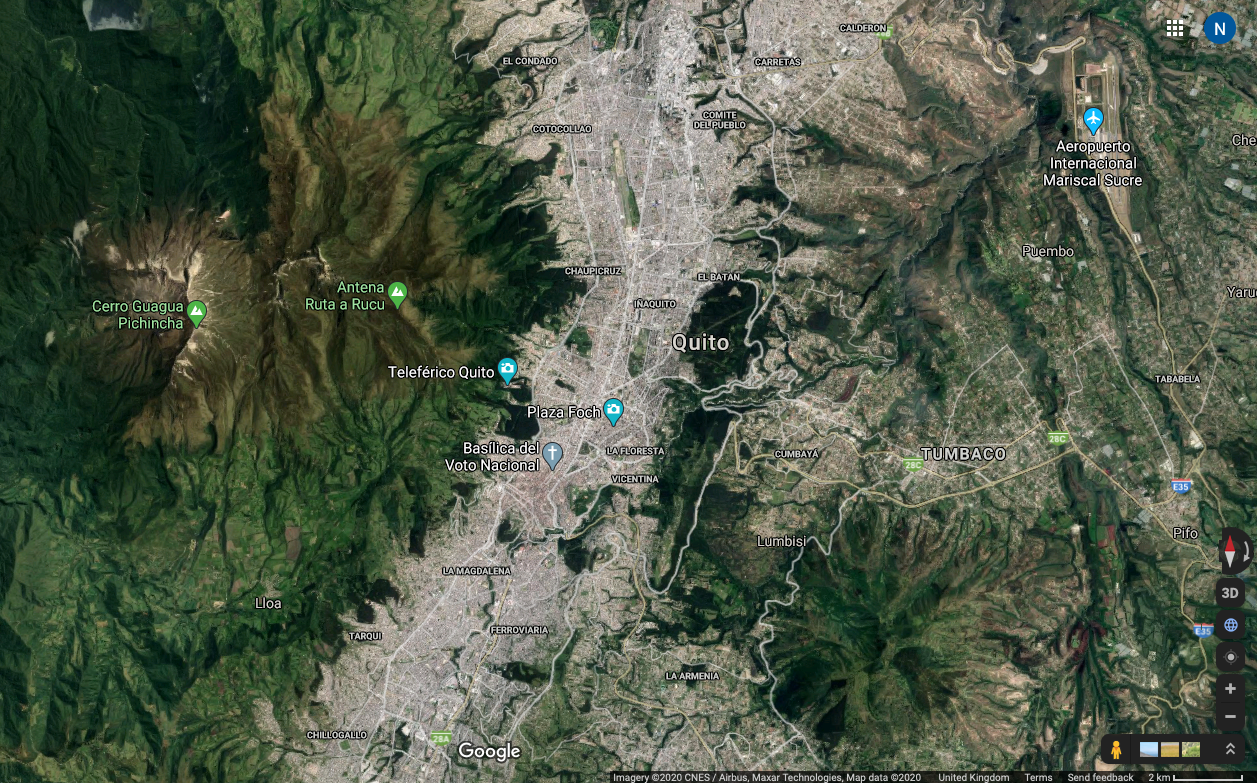
\includegraphics[width=0.8\textwidth]{Google Map Overview of GP and Quito.png}
    \label{fig:fig1}
    \caption{Screen shot of Guagua Pichincha, looking North with Quito, capitol city of Ecuador, dominating the lowlands to the East. Image taken from Google Maps on June 23rd, 2020. }
\end{figure}

Our research question for this exercise: \textbf{How many people are at risk to the different eruptive products of Guagua Pichincha Volcano, Ecuador (Figure \ref{fig:fig1})?} I selected this question for a few reasons. The first reason is that, on the whole, this question is pretty easy to answer using GIS. This is because the datasets required are quite readily available, and require minimal manipulation to get in a use able form. However, the challenge of this project is the fact that it requires non-geological data which geologists are often loathe to find. It also takes place in an area of the world many people in the McGill SEG chapter may be unfamiliar with, and the metadata is even in another language! Further complicating things is that the geological information available is locked away in non-georeferenced datasets. So while this question is easy to address at a birds eye view, if you want to answer it \textbf{you need the a full appreciation of the core "GIS Toolkit," which is the goal of this course.}

\subsection{Transferable Skills}

Based on these goals, Exercise 1 should impart several important skills that will be useful in any GIS project:

\begin{itemize}
  \item Project Planning
  \item Locating Data and Understanding Metadata
  \item Importing Data
  \item Setting Up a QGIS Workspace
  \item Defining a Coordinate References System (CRS) and Projected Coordinate System (PCS) for your Project
  \item Reprojecting Data
  \item Georeferencing a Base Map
  \item Calculating Errors
  \item Geoprocessing
  \item Spatial Statistics
  \item Styling Raster and Vector Data
  \item Visualizing Geographic Data
\end{itemize}

\subsection{How To Use This Guide}

This guide is meant to accompany the live lectures and demonstration associated with the \textbf{GIS for Geoscientists workshop}. This workshop was first offered to the Student SEG Chapter at McGill University in June of 2020, and takes the form of four 2-hour interactive instructional sessions. In line with the Objectives and Skills I highlight above, this guide is meant to serve as a permanent reference for workshop attendees. This guide will not be a complete replacement for viewing and participating in the live workshop, but aims to provide an image-packed how-to for the beginner level skills we learned in Session 2. If this is your first time encountering the exercise because you missed the workshop, or you are a compete beginner with GIS, I recommend following the guide as is. I also recommend having the first and second workshop lecture open to supplement what you are working on. If you attended the workshop, or you are a proficient user who needs specific information about a particular task, feel free to move through the guide in your own order. The tasks don't need to be completed in the order laid out by me in all cases. Enjoy the guide, and let me (Nick) know if you have any questions or comments on GitHub! Happy GIS-ing!

\section{Project Panning + GIS Motivation}

The first topic addressed in the lecture was the need to properly articulate WHY you need GIS, and WHAT you intend to get out of a GIS analysis. This is similar to any self-directed critical question you'd ask yourself in research, e.g. "what am I hoping to achieve with this particular tool?" The reason I want to be up front about this need is because like any other research technique, GIS involves training, and you want to be sure the time invested in using GIS is invested wisely. Some of the operations I show you in this guide can be performed in other software suites - particularly using Python and R. If your goal is limited in scope, it might be worthwhile to see if any of your other skill-sets will allow you to answer the same question. 

With that preface in mind, there are several obvious reasons why you might plan a project with GIS in mind. When you want to take a range of spatial datasets, overlay them, analyze some feature(s), and produce a well defined, beautiful map, Python's command line (or cell-by-cell interface in case of an IDE like Jupyter Notebook) may not be the most logical and effective way to structure your project. One of the clear advantages of GIS software is its interface, which allows the user to control every aspect of the data in question, most especially its appearance. This interface is at the same time a big barrier for people getting into GIS - the first time you open QGIS, you'll be overwhelmed by the sheer number of menus, buttons, and tools at your disposal. This is where time investment, mentioned in the previous paragraph, really comes in. In my experience, half the battle in a GIS project is finding the right button or menu, which is often buried in some obscure interface. But the fact that there are so many ready-made tools and options in a software like QGIS adds to the value of the software. Rather than defining a spatial analysis procedure from scratch and formatting the resultant map using something like \textit{matplotlib}, GIS lets you does a lot of the background work for you. 

Another advantage of a GIS is its ability to contextualize your data. Say you are a geochemist, and you've spent months in the lab analyzing a suite of elements in your samples. After all that hard work, you will naturally want to extract the maximum scientific value out of your results. This can of course be done without a GIS, but as we shall see, overlaying your spatially-defined sample data with GIS layers describing the natural hazards, topography, hydrology, and demography in your study area can provide a much richer picture of the impact your results on the systems + people it comes from. If you had analysed whole rock chemistry of scoria from different eruptive periods at Guagua Pichincha, or modeled the record of earthquakes below the edifice over a long time period, you will be able to say with certainty what impact the hazard you've identified will have on the populations affected. This analogy extends beyond volcanology of course; you should be able to see the same spatial dimension in any geological dataset, and as soon as that dimension is visualized the apparent usefulness of GIS should jump out. Finally, I can't end this discus ion without highlighting the power of GIS to advance your career. In the private and public sector, having a GIS skill set marks you out as a great candidate for a host of jobs both in the field and in the office. Given the time and experience it takes to master GIS workflows, companies and organizations will value you for this skill, which is applicable well outside geology. In fact, GIS is arguably more important than many highly technical geological skills we learn in a PhD, as they are applicable in some many non-academic applications: think Google maps, software development, COVID tracking, environmental remediation, hydrogeology, subsurface exploration, etc. 

Having laid out all these considerations as to WHY you might choose to sue a GIS, the next logical step is to ask: "Where do I start?" The first point for any scientific investigation is your research question. Thanks to the discussion in the previous section, we already have that established in our case. It's worth adding that this question comes to us because Guagua Pichincha is only 10 km. W of Quito, the capitol of Ecuador. Depending on the nature of the hazards posed, we can hypothesize a large proportion of the population are under threat from this volcano. Our next step after framing our question is to think about what stage of our analysis GIS will factor into. GIS is incredibly helpful when planning field work, as the mapping functions should make obvious. However, GIS can also add that "context" to your data I mentioned before. Even if you don't need to do any exploration or data, the map-making functionality alone makes GIS essential for manuscript figure generation. Based on these features, we can break the "stages" of GIS applicability into a \textbf{Early Stage} (planning, querying available data, generating a research question), \textbf{Analysis Stage} (spatial statistics, validating analyses, contextualizing results, modeling), and a \textbf{Post-Analysis Stage} (figure creation, map making, preparing data for publication).  

Once we have the WHY and the WHERE, we need the WHAT and HOW: what specific steps and information do you need to set off on this project. This guide will examine the search for data and the specific steps for GIS analysis in great detail. However, two more factors can be brought into our project plan. The first is follows on from my lecture in Session 1, and that's the coordinate/projection system we are going to use. This will also be treated in some detail below, but regardless of which stage of GIS analysis you are in, this needs to be one of the first things thought about and decided upon. For now, we will put a pin in that as we search for the data we need and get our GIS work space set up for the first time. The second factor is something that comes with experience, and that's an early "sketch," of the steps we will need to take in our project. For example, I know looking at our research question, I'll essentially need to compare the areas of two vector files: the vector file describing the spatial footprint of the hazard, and the vector file describing the spatial distribution of the population. This operation is called an \textbf{Overlay} and can be accomplished with several different \textbf{Geoprocessing} tools, all with applicability in different situations. Like anything else, this forecasting of the tools needed to answer our questions only comes with practice. I'll share some more thoughts on this topic at the end of this document. However, for now, we are ready to begin our GIS journey. 

\section{Downloading and Installing Software}

Our choice of software for this workshop is QGIS, formerly known as Quantum GIS. QGIS is one of the most popular open-source GIS platforms, developed by a large team of professional + volunteer software developers since 2002 through the Open Source Geospatial Foundation (OSGEO: \href{https://www.osgeo.org}{https://www.osgeo.org}. QGIS is packaged into disk installers that work on all operating systems. At the time of writing this, I am using QGIS 3.10.6-A Coru\~na - this is the current Long Term Release (LTR), which will be supplanted by QGIS 3.14-Pi sometime in the next 6 months (see Figure \ref{fig:fig2}). If you are on a Mac (like me) the download disk should show multiple installers after opening. These should be installed in the following order: (1) Python-3.8, (2) GDAL-3.1, and then (3) QGIS-3.10.6. Python and GDAL must be installed prior to QGIS - QGIS has dependencies that link to both of these programs. If you are uncomfortable updating Python at this stage (this will likely only affect avid programmers), I recommend following the isntrucitons from this \href{https://github.com/rafdouglas/qgis_desktop_docker}{older docker build of QGIS 3.4/3.6}

\begin{figure}[htbp]
    \centering
    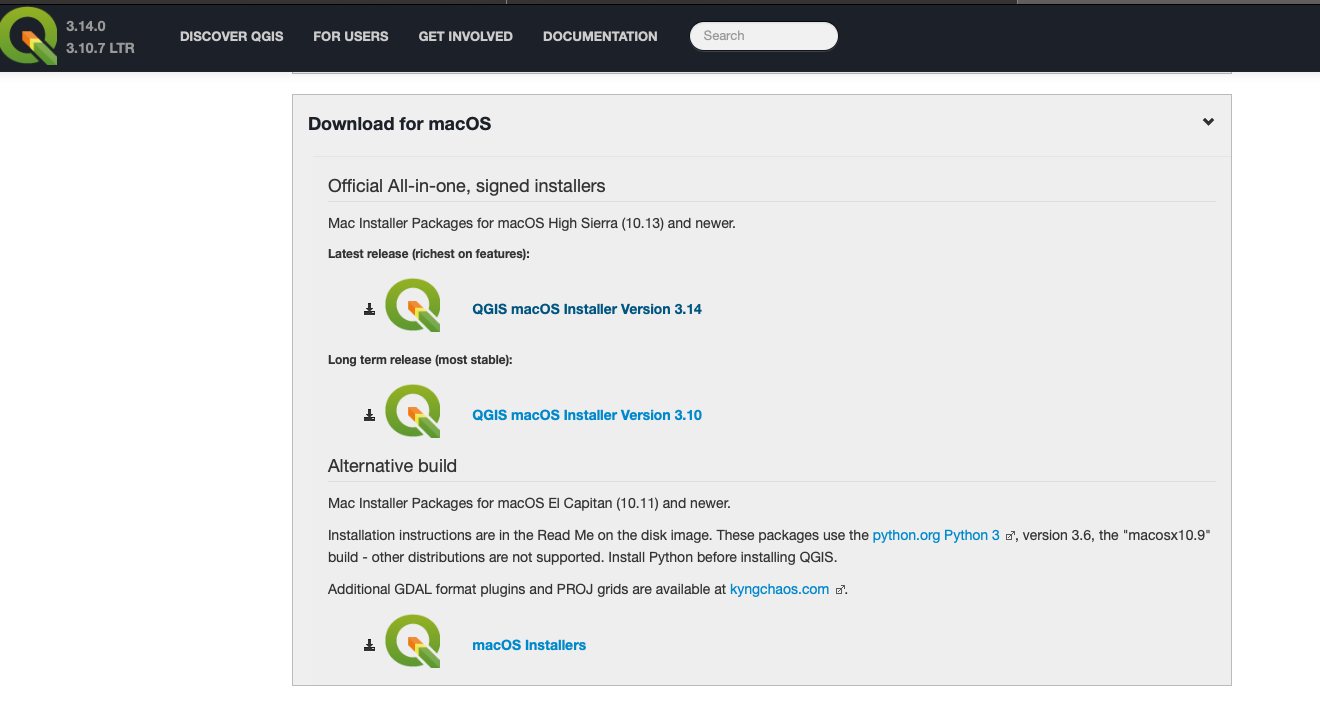
\includegraphics[width=\textwidth]{Figure2_Downloads.png}
    \label{fig:fig2}
    \caption{Screen shot of QGIS download page for Mac. As mentioned in text, this guide is based on the LTR 3.10.6-A Coru\~na. See QGIS docs for more details on versions and installation process.}
\end{figure}

There have been some dependency problems with GDAL 3.1 and QGIS, both in my experience and as reported on the forums. These are likely to be cleared up soon after this guide is published. However, in the event they aren't, it might be wise to install \textit{conda} or \textit{pip} versions of GDAL in their own environments. Using the Terminal on Mac, type one of the following:

% Can actually import code here:  \lstinputlisting[language=Octave]{BitXorMatrix.m}
\begin{lstlisting}[language=Python]
    conda install -c conda-forge gdal 
    #OR
    pip install GDAL
\end{lstlisting}

One of the recommended installation steps is to fix the paths to GDAL and Python on your system. QGIS sometimes has trouble finding these directories, and by fixing these paths you make it easier for the program to find the right modules. Figure \ref{fig:fig3} shows a screenshot of the pathing needed; to get to this menu, click the dropdown menu title 'QGIS', and select Preferences > System. Under System there is a collapsible menu called "Environment. Here you can enter your paths. You want to select 'Prepend' for APPLY, and 'PATH' for Variable. Enter the paths as described here if you use Mac. The installer will likely have different pathing instructions for Windows and Linux systems, but the essence of these instructions are the same. 

\begin{figure}[htbp]
    \centering
    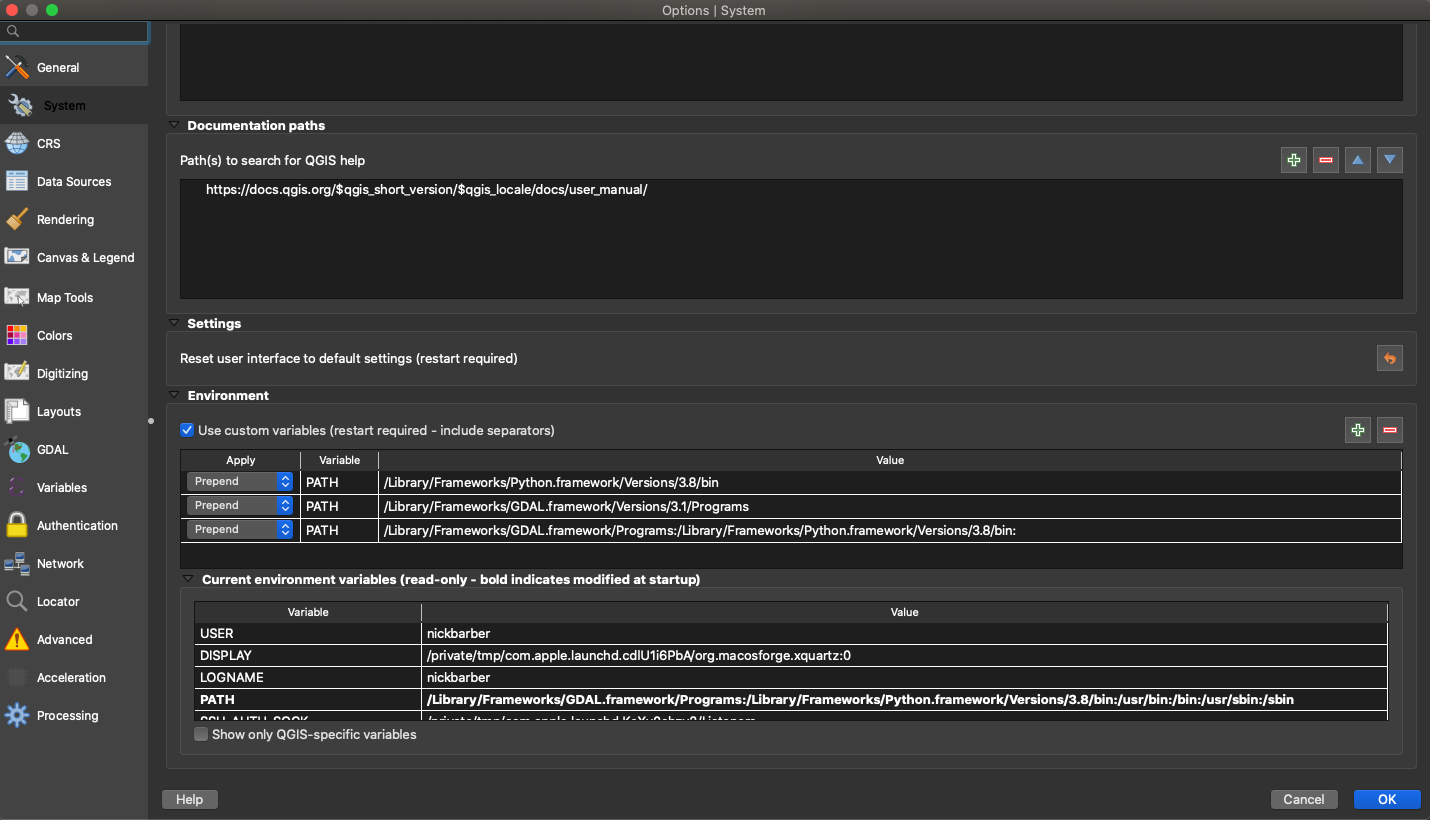
\includegraphics[width=\textwidth]{Figure3_Environment_Paths.png}
    \label{fig:fig3}
    \caption{Environment Menu under QGIS > Preferences > System dropdowns. If you are a Mac user, copy these three Prepend paths to map your QGIS properly. Othrwise, you might experience Python errors at start up.}
\end{figure}

\subsection{Plugins}

For this exercise, you will need the following plugins. These can be found in the main menu drop down (see Figure \ref{fig4}) under Plugins > Manage and Install Plugins. Notice how some plugins are marked as a "Core Plugin," with a cyan banner upon selecting. Long ago, these were standalone plugins, but have since been folded in as core features of QGIS. We will be using many of these core plugins as well:

\begin{figure}[htbp]
    \centering
    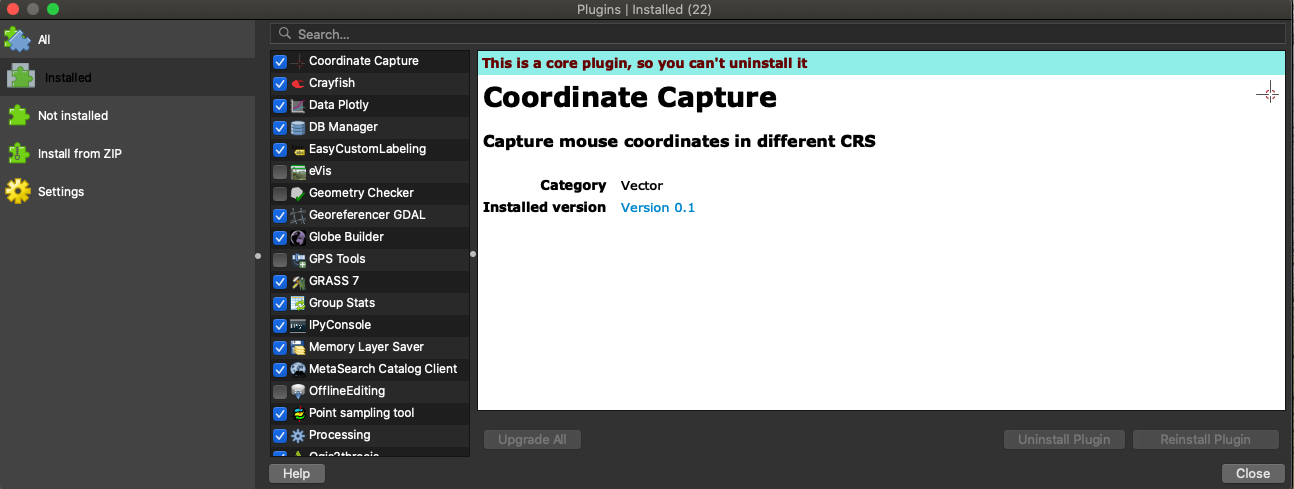
\includegraphics[width=\textwidth]{FIgure4_Plugin_Menu.png}
    \label{fig4}
    \caption{My 'Manage Plugins' Menu. Notice how many more are enabled than you will need for this exercise; many of the plugins are useful but not to our current goals. Contact me if you have any questions about what some of these plugins do.}
\end{figure}

\begin{itemize}
    \item \textbf{Quick Map Services}: Should be a core plugin now, but will allow you to upload base maps. Base maps don't have geographical information per se, but they work as a good "base layer" for any map.
    \item \textbf{Globe Builder}: Useful plugin for larger scale maps, let's you create pseudo-3D spherical map projection centered on your data. Great for data visualization.
    \item \textbf{Easy Custom Labeling}: One of the most useful plugins for map making. Allows for detailed and intuitive user control of labels. Labelling is a famously painful procedure in GIS software, and this is one of the best tools I've found to make my labels consistent and appealing.
    \item \textbf{Memory Layer Saver}: If you are going to sue Easy Custom Labeling, I strongly recommend having this plugin enabled as well. Easy Custom Labeling outputs a unique data type, called a memory layer, that will disappear after a particular map session is over. Memory Layer Saver allows this layer to be saved and preserved for future sessions, guaranteeing map consistency as a project evolves.
    \item \textbf{GroupStats}: Simple but incredibly intuitive, this plugin lets you calculate statistical features of vector layer attributes, and export the results to a CSV. For a mroe detailed overview of its functionality, see: \href{https://anitagraser.com/2013/02/02/group-stats-tutorial/}{https://anitagraser.com/2013/02/02/group-stats-tutorial/}
    \item \textbf{QuickOSM}: A very sueful built in tool that helps users locate gernic, pen soruce datasets for mapping. Builds simple queries to access the publicly maintained data sets in the Open Street Map 
\end{itemize}

\section{Opening QGIS for the First Time}

Upon installation of QGIS and the recommended plugins, you are left with a bewildering array of menus, buttons, and windows. Like learning to read, the symbols and menus seem incomprehensibly arrayed, with no logic or order. It can be very overwhelming! Thankfully, this guide and future exercise will slowly introduce you to the important menus. My hope is that by the end of this exercise, you'll be able to locate some of the essential, day to day tools and functions with only a minor amount of googling. 

Through the previous few sections, you've already met a few menus. These have been accessed via the \textbf{Menu Bar}, a row of drop-down menus at the top of your screen. Below the Menu bar, is the array of \textbf{Toolbars} that can be enabled and disabled for view by selecting the Menu option "View", followed by "Toolbars," near the bottom of available options. These toolbars can be moved at will by clicking the vertical dotted lines separating each tool bar (see Figure 5). The center of the screen is taken up by the \textbf{Map View}. This is your work space, where all mappable elements will be displayed. To the left and right of the map view are \textbf{Panels}; these will be discussed in turn, but they are the menus that will allow you to visually control most of the features you care about with your map. Finally, the bottom of the screen has a greyed out area called the \textbf{Status Bar}, where details about the coordinates of view, scale, degree of rotation, projection system, and search bar are found. 

\begin{figure}[htbp]
    \centering
    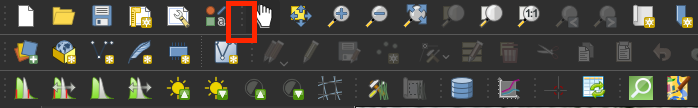
\includegraphics[width=\textwidth]{Fig_6_Toolbars.png}
    \label{fig6}
    \caption{Zoomed in screen shot of toolbars at the top of my QGIS interface. The vertical dotted lines used to move toolbars is highlighted with a red box.}
\end{figure}

For a more detailed visual tour, please see the QGIS documentation: \url{https://docs.qgis.org/3.10/en/docs/user_manual/introduction/qgis_gui.html}

\subsection{.qgz: The Project File}

Before moving on to the main part of this exercise, it's worth spending a moment to highlight the file structure that's going to be your home for all the fun analyses you are running: the Project file. This file type is essentially your container for every other file you are going to plot, analyze, combine, and map in the course of a GIS session. When you first open QGIS a blank project file is all you have the option to save. This file has the extension \textbf{.qgz}, and can be saved alongside your actual data files. Like other programs, you can take features of your project file, and save them as templates for future analyses if you like the way you structured a particular map. Two important aspects of a project file need to be made clear. First, a QGIS can only operate one project at a time; it's not possible at the moment to have multiple projects open like you would in Adobe Illustrator or Inkscape. Second, \textbf{saving a project file does not save your actual data, analysis, models, or maps.}. 

This second point is critical, and is often confused by new users. To illustrate this problem, I'll pose a simple and very realistic scenario illustrating what I mean. Imagine: after doing some work and making a pleasing looking map, you will naturally hit the "Save" button in the upper left icon menu, exit out, and continue with your work. Weeks later, you will reopen QGIS and immediately be met by a scary menu, telling you that QGIS can't find your files! This situation will often be met by smattering of curses, and may lead to you redoing a lot of your work. So what went wrong? What probably happened is that in the ensuing weeks since you started your .qgz file, you did some reorganizing in your hard drive and moved some of the shape files or raster files used for your map to another folder. Unlike many other applications, your project file and its contents are linked together very loosely. What this means in practice is that when you save a project file, you are essentially saving 1) styles and colors you've sued to make your map 2)the order of appearance of different layers 3) the projection system used 4) other metadata, but crucially not the actual files themselves. Those files exist in a unique portion of your hard drive with their own file path, so when you moved those files to a nice, orderly sub-folder AFTER the creation of your initial project file, QGIS essentially "lost track" of the data. 

All you need to do to fix this issue is to click on the files that are throwing an error, and find them in your hard drive (easier said than done when you come back to a project you haven't opened in six months!). The good thing about this setup is that even if you break, delete, or make a change you don't like to a project, the underlying data can still be saved. Given all this, I don't want you to leaver this section thinking that the lesson is here is not to avoid saving or caring about a project file. Rather, document for yourself where you've stored everything, and keep track of what changes are being made. The utility of a project file will become more apparent later on in this Exercise. For more information, see \url{https://docs.qgis.org/3.10/en/docs/user_manual/introduction/project_files.html}

\begin{figure}[htbp]
    \centering
    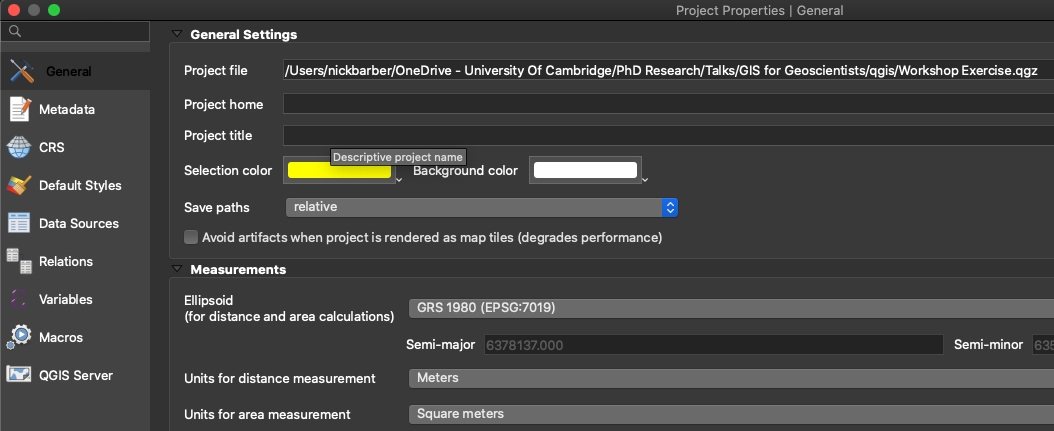
\includegraphics[width=\textwidth]{Figure 5.png}
    \label{fig5}
    \caption{Project file directory and options. This menu is from the "Properties," option, accessed from the "Project" drop-down in the main menu bar.}
\end{figure}

\section{Finding GIS Data}

After identifying your research question, installing QGIS and relevant plugins, and familiarizing yourself with the interface, you will probably be left staring at the screen, wondering: where do I go from here? This initial paralysis is understandable. Despite all the wonderful features of QGIS we are going to use to understand Guagua Pichincha, there's no road map readily available on where to go to find the data you need. We are faced with two problems when thinking about what data we need. The first problem is the classic, "I have data, but how do I get it in to GIS?" This is one of the most common questions I get asked. Never fear; I will address this problem in great detail in the next section. More immediately, we need to co consider our non-geological needs. Specifically, our need for supporting information to achieve the stated goals of this exercise. What do I mean by supporting information? To take our research question seriously, we need a lot of information whose source and scope may not be immediately obvious. This information includes the spatial location and scale of the city of Quito itself (infrastructure, buildings, municipal boundaries, population statistics, etc. ) and the surrounding environment (weather, topography, hydrology, etc.). 

Without the aforementioned mythical road map to data, this can seem like a very difficult problem to solve. Fortunately, many years of facing this same experience myself has led me to collate a host of resources that will make your first attempt at this easier. I provide URLs to each of these resources in turn in my Second Lecture, but I will provide a more detailed summary of each data source here. 

\begin{itemize}
    \item \textbf{GeoData @ Tufts} (\url{https://geodata.tufts.edu}): An all purpose data clearinghouse for spatial data. This website essentially references open source data from around the world, covering needs like base maps, population, infrastructure, climate, and many others. Coverage is generally pretty good the world over. Metadata linked to downloads provides the relevant "key" for interpreting what different fields mean. Also linked to a companion site through Harvard (\url{http://hgl.harvard.edu:8080/opengeoportal/})
    \item \textbf{Mineral Resources Online Spatial Data} (\url{https://mrdata.usgs.gov/general/map-global.html}): Useful data source for any economic geology needs. Curated by the US geological Survey (USGS), this data set not only includes regional scale spatial information about ore deposits, but also more detailed geological information (global geology maps) and commodity information (grade, tonnage, ownership, etc.). This data source is a must use for specialists in Economic Geology.
    \item \textbf{NASA GES DISC} (\url{https://disc.gsfc.nasa.gov}): One of the highest fidelity data sources I've found. Climate, atmospheric, weather, and environmental data at high resolution for most of the globe, all sourced from NASA satellite missions. Requires a free account to manage downloads. File format is atypical for GIS uses; you will need to use an .HDF to GeoTIFF conversion tool provided by NASA to port these datasets into QGIS (HDF can;t be read by QGIS, but GeoTIFF can). More details on how to perform this conversion can be found here: \url{https://gis.stackexchange.com/questions/65875/translating-modis-hdf-to-geotiff}. Two common conversion solutions: use command line code from the GDAL library ("gdal-translate" function - this is the easiest solution but only if you are comfortable with coding), or use NASA's own conversion tool: \url{https://wiki.earthdata.nasa.gov/display/DAS/Downloads}
    \item \textbf{USGS EarthExplorer} (\url{https://earthexplorer.usgs.gov}): This is probably the data source I use the most. Like the NASA GES DISC, this website requires you to create a free account, as well installing a "download manager," called the BDA Manager for big files. Contains staple satellite datasets like LANDSAT, Aerial Imagery, Digital Elevation Models (DEMs), Land Use, Vegetation Index, Radar, UAS, and many more. We will use this data source in our exercise here. I highly recommend bookmarking this site for future use!
    \item \textbf{Land Use GeoPortal} (\url{https://landportal.org/book/data}): Nonprofit spatial data service that provides land use, land ownership, property rights, and social justice oriented data services. Coverage isn;t necessarily global, but very specialized for particular social issues e.g. indigenous land disputes in South American. Great data source for integrating social information with your geological maps. 
    \item \textbf{ArcGIS Hub} (\url{https://hub.arcgis.com/search}): Very Similar to the Tufts service: provides a curated list of datasets from all over the world. Serves a variety of purposes (infrastructure, environment, boundaries, transportation, etc.), and datasets are present in many major languages. While this service is maintained by ESRI (the parent company of ArcMap), the data is still freely available to download. 
    \item \textbf{Natural Earth} (\url{http://www.naturalearthdata.com/downloads/}): Go to open data source for base maps, showing municipal, national, and physical boundaries at different scales. This data source is used by some mapping services as their default base map. Shape files and raster data can be freely downloaded from the site without an account.  
    \item \textbf{NASA Socioeconomic Data Center} (\url{https://sedac.ciesin.columbia.edu}): Similar to the Landportal resource, in that it links environmental and socioeconomic data. In contrast to Landportal data has less social context, and has better global coverage thanks to satellite data integration. Requires registration with a free account to download. 
    \item \textbf{OpenTopography LIDAR Data} (\url{https://opentopography.org}): Niche use service that provides LIDAR data for a variety of purposes. Unfortunately, open source LIDAR coverage has limited global coverage, and the data here is restricted mostly the the US, Canada, and Western Europe. Downloads work best using Chrome or Firefox browsers.
    \item \textbf{UN Environmental Data Explorer} (\url{http://geodata.grid.unep.ch}): Multi-scale sociological, business, environmental, climate, and humanitarian data. This repository is old and not well maintained, but contains good historical information. 
    \item \textbf{Integrated Population and Environmental Data (IPUMS Terra)} (\url{https://terra.ipums.org}): Similar to LandPortal and NASA Socioeconomic Data Center. Provides up-to-date health and environmental data. Well maintained, well curated. 
\end{itemize}

For our exercises, GeoData @ Tufts and USGS EarthExplorer will be our primary data sources. Besides the geological information brought in from the literature, almost every layer we use will be from these two sources. However, I encourage you to explore what each data repository has to offer when pursuing your own research. The data we need to complete this exercise includes the two main categories listed below.

\textbf{Shuttle Radar Topography Mission 1-arc Second Elevation Data} (USGS EarthExplorer): SRTM DEMs are some of the most widely used elevation datasets in GIS. They aren't ideal for incredibly detailed, high resolution work, but they are essential for most regional scale analyses. As we'll see, the resolution is more than good enough to look at G.P. in great detail. To download, you need to select an area of geographic interest (e.g. the city of Quito) when you first open Earth Explorer using the "enter Search Criteria" Menu. Then navigate to the "Data Sets" tab (see Figure 7), and navigate to "Digital Elevation." Click on this menu, and then click on the sub-menu "SRTM." In most cases, you'll use "SRTM 1 Arc Second Global" as your data source. After checking the checkbox next to the data name, navigate t the bottom of the page, and click the button "Results >>>", which will lead you to the "Results," tab. Next to the icons showing available data sources, you can manually download each file. \textbf{These downloads are raster data types}. The actual format and import procedure for these files will be discussed later, but for now, regard them essentially as pixelated image files. Note: you must be logged in with your free account to download these files. Where you are downloading many files, you will need to sue the USGS' BDA application manager: \url{https://www.usgs.gov/media/images/earthexplorer-bulk-download-application-bda}.

\textbf{Ecuadorian Base Layers} (GeoData At Tufts): Start by typing "Ecuador" into the location search bar. \textbf{We may need a variety of layers to answer our research question. The layers we are looking for are: Roads, Airports, Coast, Rivers, Population Census, Province, Canton, and Parroquia.} These layers will let us assess the impact of volcanic hazards on the population of Quito, as well as any relevant infrastructure. Some of these layers may not end up being of much analytical use, but layers like the Coast or Province/Parroquia boundaries will prove incredibly helpful when making our final map. You can search each of these terms in the "What" search box after narrowing the search region to Ecuador. Once you find a layer of interest, you can see what it looks like by ticking the "View" box for that layer. When you are happy you have selected the appropriate file, you have to add that layer to your cart (Figue 8). You do this by selecting the Plus symbol to the left of the file name. When successfully, added, the Plus sign will change to a green check-mark. Once you have completed your selections, navigate to the "cart" tab, and select Download. You will be prompted to select a data download format. Make sure you select "Shape File." The resulting download may take several moments, and all result swil be dumped into one ZIP file. \textbf{Unlike the raster DEMs from EarthExplorer, these files usually have a vector data type.} This means that the file structure is more complex. This will be explained in more detail in the next section, but for now, each "layer" you added to yor cart is actually composed of seven separate files that stitch together when loaded into QGIS to make one layer. \textbf{Never delete one of the subsidiary files associated with a shape file! And always hang on to the relevant XML file; this contains the metadata and key for any unfamiliar terms.}

\begin{figure}[htbp]
    \centering
    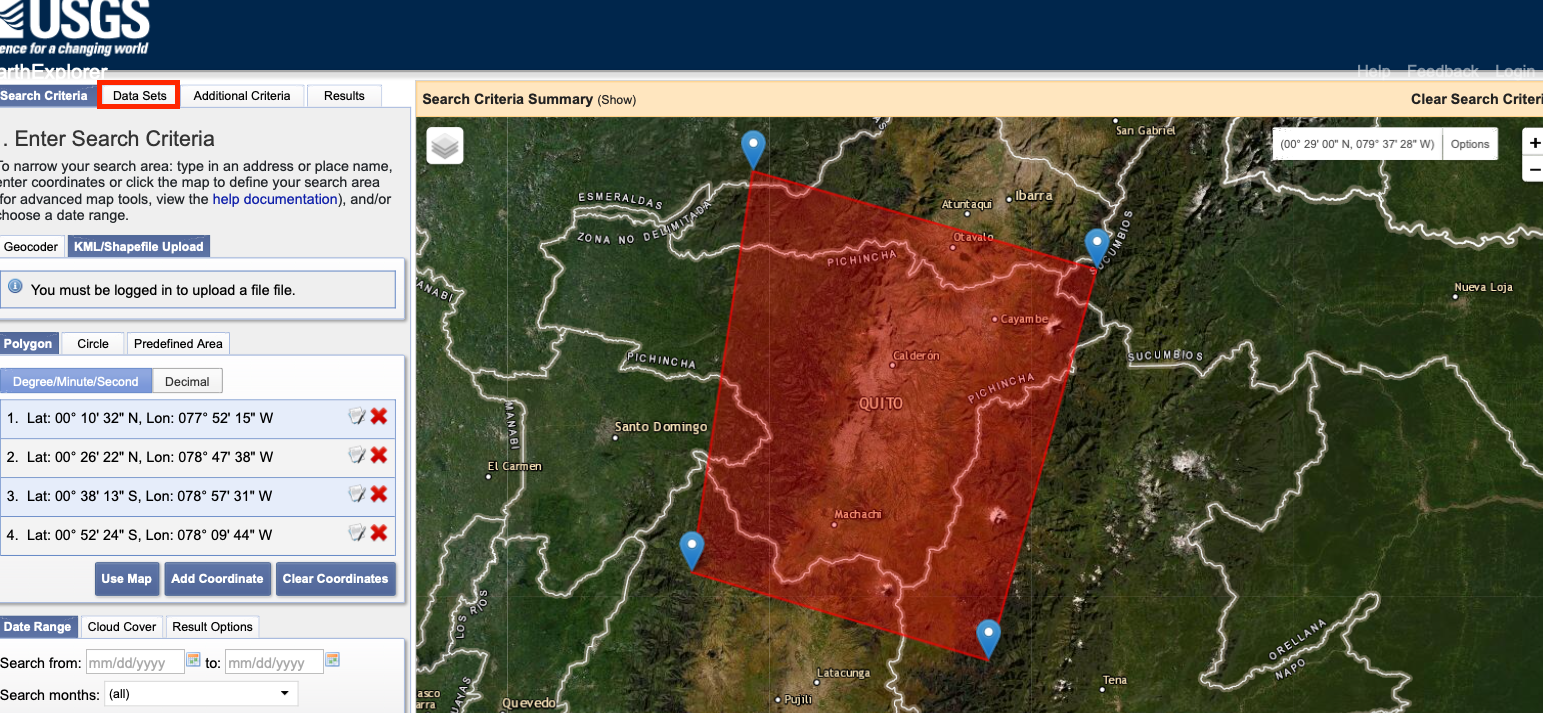
\includegraphics[width=\textwidth]{Fig_7_EE.png}
    \label{fig7}
    \caption{View of Earth Explorer interface after I've selected the Quito area as my Search region. I created this red box by zooming to the scale I wanted, and selecting the button "Use Map" in the "Polygon" menu. The "Data Sets" tab mentioned in the main text is highlighted with a red box.}
\end{figure}

\begin{figure}[htbp]
    \centering
    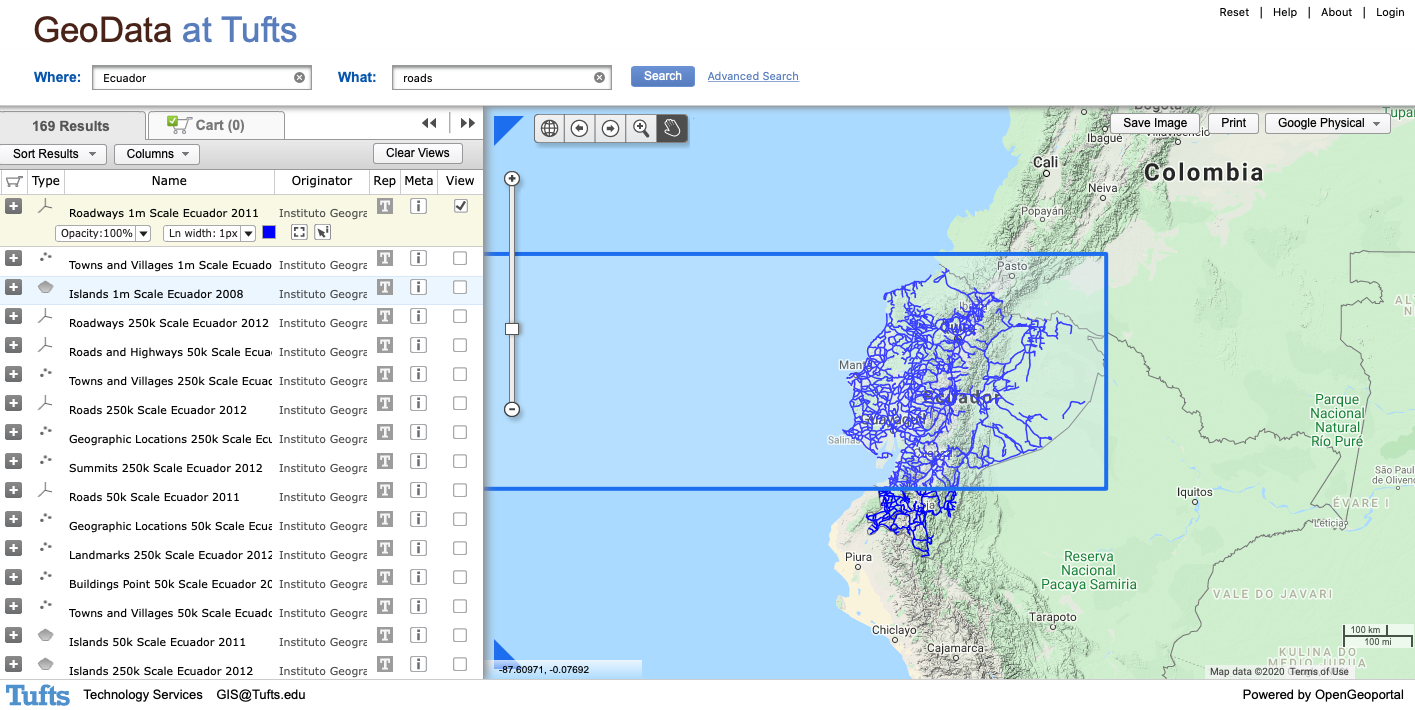
\includegraphics[width=\textwidth]{Fig_8_Tufts.png}
    \label{fig8}
    \caption{Screen shot of my selection of the 1m scale roadways layer from GeoData Tufts. The relevant selection and download options can be seen on the left hand side.}
\end{figure}

If you'd like to save some time, the ready-to-use files are available via the GitHub home page for the course. Simply download the course data, and navigate to the "qgis" folder. Relevant files are stored in appropriately named subfolders. Now having written > 5000 words about QGIS in theory, it's finally time to import some data and start our exercise! 

\section{Importing Data}

This first step in our GIS journey will be a good opportunity to introduce some key features of the software. Particularly, this step should familiarize you with some of the common layouts and processes you need to follow when accessing QGIS tools. Importing data may seem trivial, bit given the plethora of data types and scale we want to work with as geoscientists, it's essential we get this right! Before starting our import, \textbf{I should emphasize that this section, Section 7, and Section 8 can be worked through in any order your prefer.} I've ordered them in this way to make it easier for me to explain what to do in writing, but there is no reason you can't start by setting up your work space (Section 8), define a projection system (Section 7), and then import your data.  So follow Sections 6-8 in whatever order makes sense to you! See Figure 9 for a brief overview of the three Import functions we are going to use. 

\begin{figure}[htbp]
    \centering
    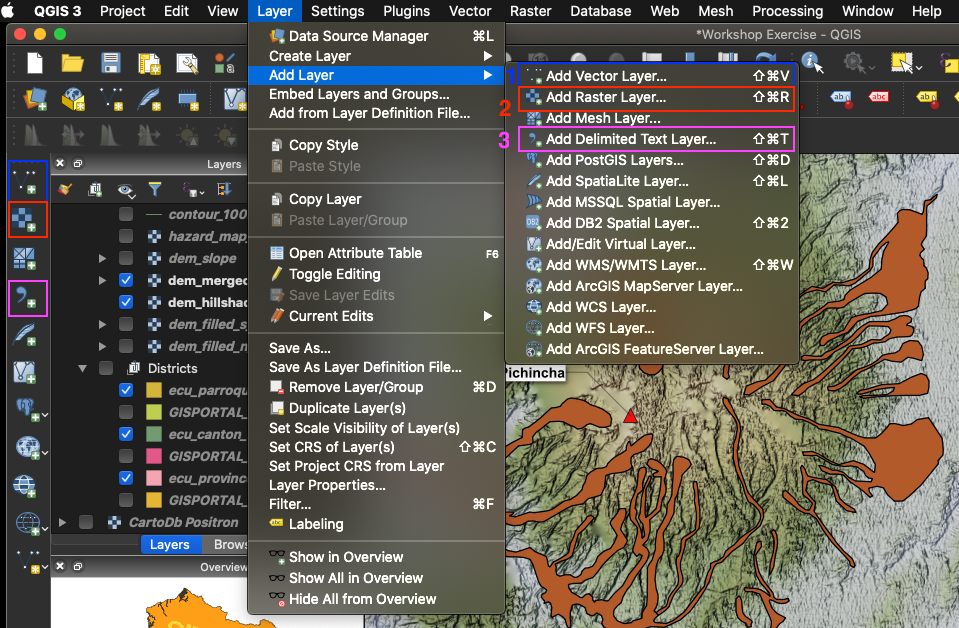
\includegraphics[width=\textwidth]{Fig_9_Import_Menus.png}
    \label{fig9}
    \caption{Overview of import functions we will use tog et our data into QGIS. These tools can be accessed using either the left hand toolbar, or the "Layer" drop-down menu. (1) Vector Import (Section 6.1); (2) Raster Import (Section 6.2); (3) CSV/TXT File Import (Section 6.3)}
\end{figure}

\subsection{Vector}

Vector data is one of the two main "staple" data formats used in QGIS, and all other GIS software. Following Menke's \textit{Discover QGIS 3.X: A Workbook for Classroom or Independent Study} (2019), vector data is "...a representation of the world using points, lines and polygons...data that has discrete boundaries." Most GIS operations, even advanced remote sensing algorithms, tend to involve some level of vector data to define the WHERE and the WHAT of the analysis being done. For us, most of this Exercise will involve manipulating vector data, and much of the data found in the "qgis" folder on the course website is vector data. Common vector data formats are the \textbf{Shapefile} (.shp) extension, which was designed for use with ESRI products but works just as well in QGIS. The other major vector data format that we will encounter is a \textbf{GeoPackage} (.gpkg), which is an SQLite Database file used widely in QGIS that comes with many advantages over traditional Shape Files. 

There are two important features of vector data that need to be discussed before moving forward. The first is the file structure, which differs depending on whether you are using a .shp or .gpkg file. Regardless of which file format you use, vector data takes the form of up to seven independnt "files", which layer together in GIS software to represent the different features of the data. The features I am talking about are 1) actual spatial location (where on earth?) 2) projection system (where on earth in relation to what reference?) 3) geographic extent (what is the shape? area? size?), 4) geometry (point? line? polygon?) 5) metadata (glossary for key terms, references), and 6) attributes. \textbf{Vector attributes} are the feature we tend to be care about most when using vector data. Attributes are typically supporting data, that populate the points, lines, and polygons defining a vector file with additional data. If we are looking at a map of the UK, where vector data with a polygon geometry is used to map the counties of the UK. The Attributes of these counties may include population statistics, demographic data, or comments (e.g. does the country contain a national park?). Attributes are stored in the \textbf{attribute table}, which we will utilize many times times in this exercise. If you are using a .shp format vector file, you are actually importing the many different "context" files which stack together to produce a single Vector file as seen by QGIS. A Geopackage is a super-efficient container that doesn't have this confusing file structure, but instead uses SQL data base structures to relate these different features of vector data. QGIS is actively promoting the use of GeoPackages, to enable easier sharing of data and to enable a more logical and transparent file architecture. GeoPackages can also contain multiple discrete ShapeFile equivalents, making them powerful and easier to share GIS data storage tools 

The other important vector data feature that differs greatly from its common counterpart, raster data, is the ability to create, append, and edit the geometry and records captured in a vector file. Much like a "shape" object in graphic design software's, QGIS lets you manually edit the spatial extent and shape of, say, a polygon defining the extent of a geological formation. More importantly, these editing tools can be used to define an "empty" vector files, and manually draw/add features where you know them to exist independently. The attributes can similarly be edited, deleted, and added to at will. This \textbf{Edting} feature will be used by us to bring the modeled extent of lahars in Quito out of the literature and into our real, interactive GIS environment. Also very powerfully, vector data, whether by shape, manual selection, or specific attributes, can be queried, filtered, and modified using a combination of custom QGIS expressions + Python code. Again, we will see how this works in great detail through the next two sessions. 

After this much discussion to importing data, you might imagine it's an arduous process. Sorry to be a let down, but it's quite easy. The trick is making sure you know what you are doing when it comes to Vector files. \textbf{After downloading the files we will use in this exercise, you import those files using the "Add Layer" feature.} DO NOT use "Create Layer," just above; this is a common beginner stumbling block (See Figure 9). But as you do this, you may ask yourself; what even is a layer? A \textbf{Layer} in QGIS is much like a Layer in Inkscape, ArcMap, Illustrator, or another other graphically oriented software. Essentially, a layer is a container linking data, spatial information, symbology (i.e., style) in a discrete object that is ordered in appearence (a layer ordered on top of another layer will be drawn on top in the Map Canvas), and \textit{unique to each project}. The uniqueness of Layers to each project was touched on in Section 4.1. We will have plenty of opportunity to familiarize ourselves with Layers and their features as we work through this exercise, so we will leave the discussion there for now. 

The protocol for importing both a ShapeFile and a GeoPackage is displayed in Figures 10 and 11 respectively. For both options, select the dropdown "Layer" > "Add Layer," followed by your format of choice (see Figure 9 for reference; you can also use the sidebar import icons next to your browser). For Shapefiles, you will usually select the ellipsis next to the "Vector Dataset(s)" drop down, navigate to the location of your file with a .shp extension in your hardrive, and then select "Add." Despite the menu looking quite different, GeoPackages work much the same way. Select "New", navigate the the .gpkg file in your hard drive, and select the specific file you want to import from the drop down bar above "New." Like mentioned earlier, this drop-down bar is there in case your GeoPackage contains more than one discrete vector file, allowing you to choose which specific features to import. 

\begin{figure}[htbp]
    \centering
    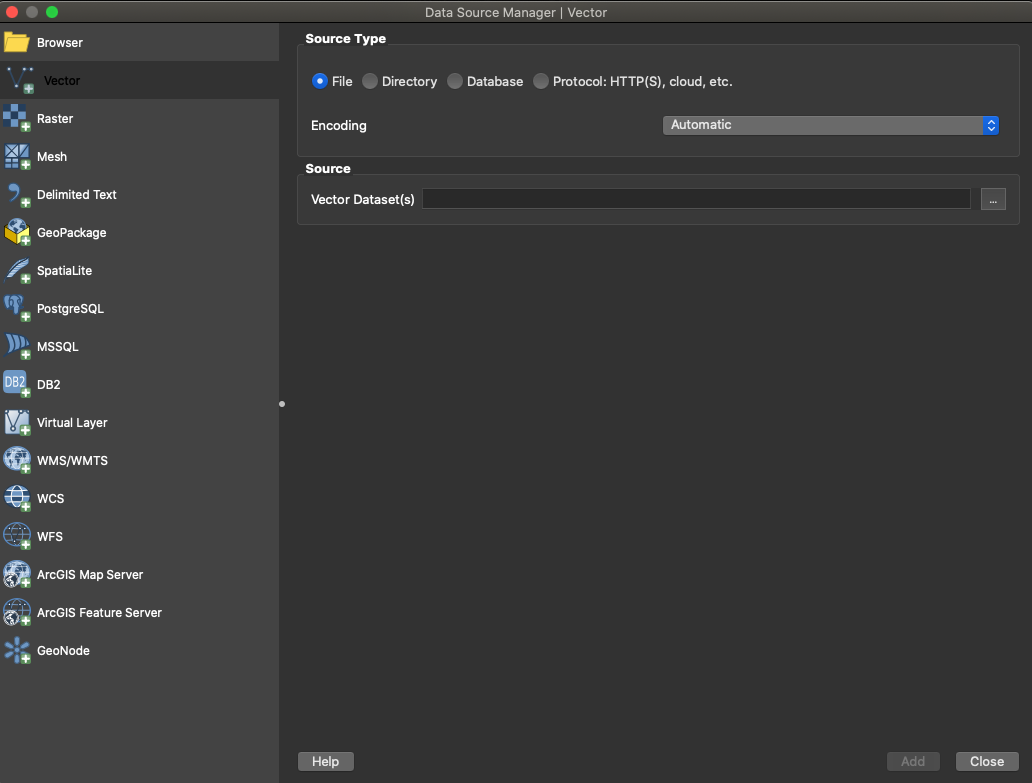
\includegraphics[width=0.8\textwidth]{Fig_10_Vector.png}
    \label{fig10}
    \caption{Simple file import window for Vector Data. usually you will sue this menu (Option 1 in Blue in Figure 9) if you are using .shp vector data formats. As you may be able to tell, whole directories and databases of vector data can be imported if you select one of the other "Source Types." For our purposes, the "File" type is what we should be using. }
\end{figure}

\begin{figure}[htbp]
    \centering
    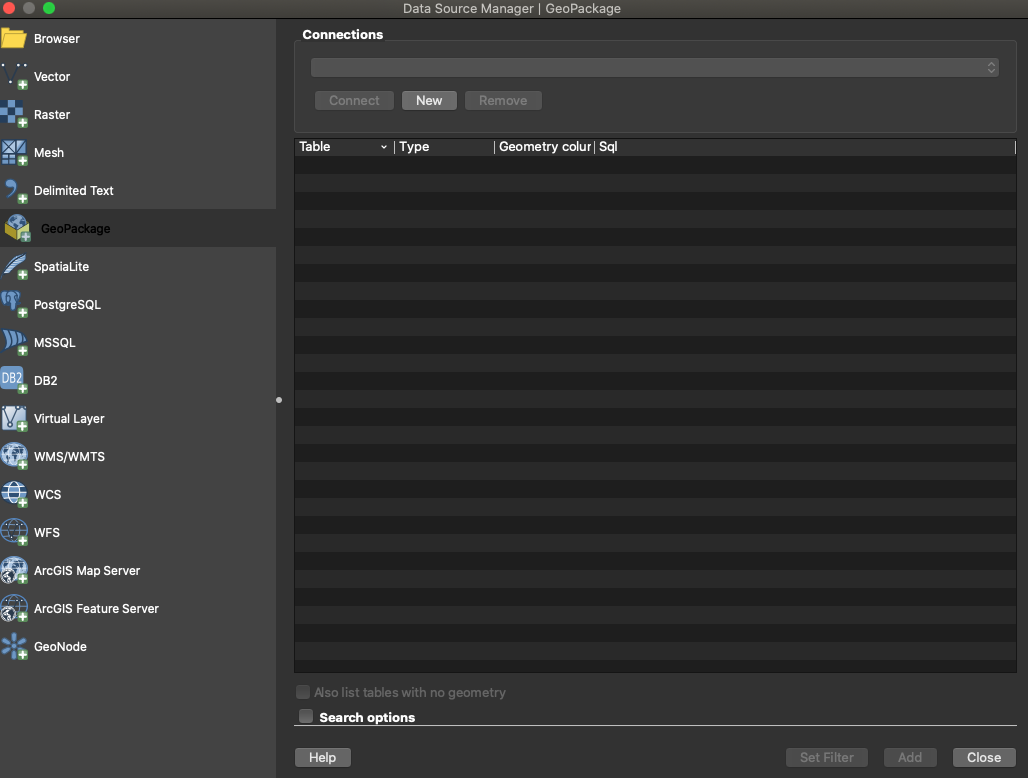
\includegraphics[width=0.8\textwidth]{Fig_11_Geopackage.png}
    \label{fig11}
    \caption{GeoPackage Import menu. Because GeoPackage's are technically SQL Database structure, the import menu resembles a database connection (if you have experience with databases). Follow the protocol in the the text to import the files you want out of your .gpkg file.}
\end{figure}

For more details: \url{https://docs.qgis.org/3.10/en/docs/training_manual/basic_map/vector_data.html}

\subsection{Raster}

Following the same reference manual as the previous section, raster data is defined as, "a representation of the world as a surface divided into a regular grid of cells. Raster models are useful for storing data that varies continuously such as an aerial photograph," (Menke, 2019). Raster data can take on both discrete (e.g. classification bands in a Landsat imaging exercise) and continuous (e.g. meteorological or atmospheric data from a satellite) values depending on the task you have in mind. Raster formats are variable, with three main types we are going to care about: (1) \textbf{GeoTIFF} .tiff - a spatially enabled version of a TIFF image file; (2) \textbf{ERDAS Image} .img - similar to GeoTIFF, but less common; (3) \textbf{Virtual Raster Dataset} (VRT) - mosaice raster that enables super efficient data storage, compilation of many files, and easy file transfer. We will mainly see format (1) and (3), with (1) being a standard for most of our small scale analyses, but (3) the equivalent of a .gpkg vector file. Across all formats, one of the most popular raster data products is the \textbf{Digital Elevation Model} (DEM), which provides gridded representations of the Earth's topography. 

In general, I find raster files to be easier to grasp from a conceptual standpoint. Similarly,  they are straightforward to import (see Figure 12). However, due to their applicability in remote sensing applications, raster datasets have a deeper layer of complexity. We won;t touch on this complexity much in this course, but I'll do my best to reference it where possible. The main point(s) of advice I'll offer with raster data concern their storage and appearance. Regarding storage, raster data tends to have huge file sizes. The base layer DEM I use for work in the Deccan Traps is greater than 2 GB. On it;s own this is a huge file, but when this file is used in analyses, disaster can ensure. This is because of one of those useful but sometimes troublesome features of GIS, which preserves the original input file while creating a unique output file of similar size. So a three step calculation can triple the memory being used to render your GIS map view. You can imagine how an iterative modle can let this get out of hand! So efficient management and rendering of raster data is paramount. 

This storage issue leads us naturally to the importance of raster visualization. Since rasters will often bu the biggest single files in your Layer browser, QGIS gives you a host of tools to make sure the high resolution grids of multiple raster layers don't overwhelm your computer's processor. These tools include \textbf{resampling}, \textbf{pyramid building}, and \textbf{scale dependent visibility.} As we load raster files, I'll try to slot in explanations of these different visualization techniques. We can also use clever tools to create \textbf{contours} from raster data, if we want to save memory and still capture a sense of the topography. Finally, the ever useful \textbf{hillshade} algorithm is going to come in handy as we try to make our map look pretty at the end of our Exercise. 

\begin{figure}[htbp]
    \centering
    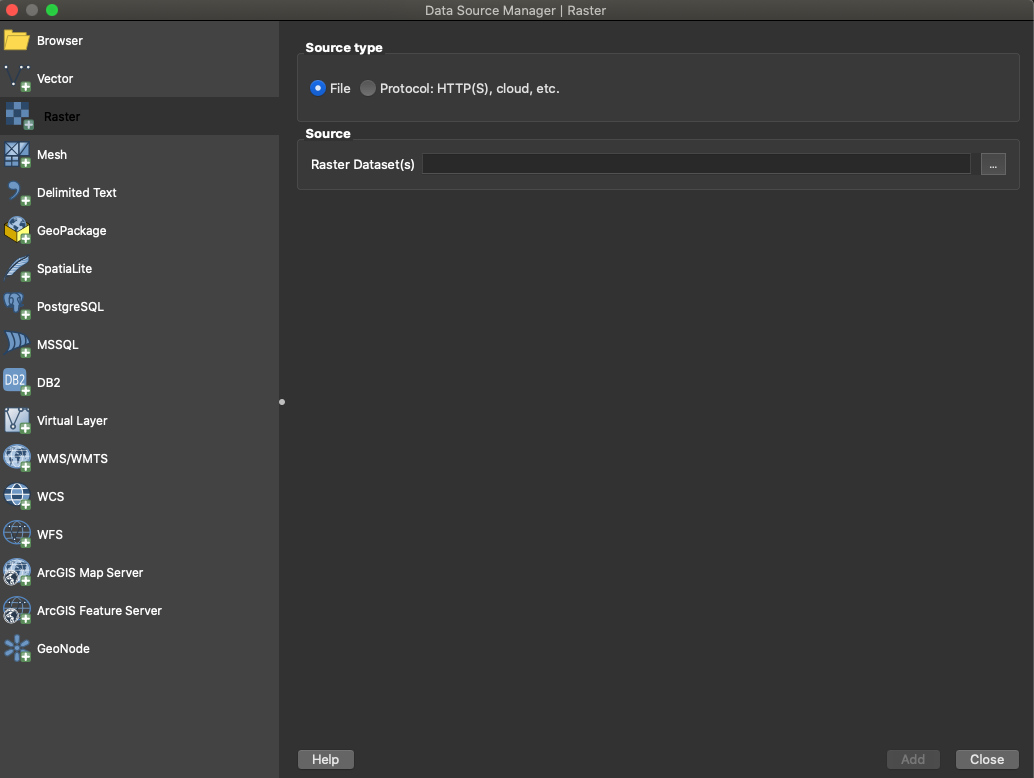
\includegraphics[width=0.8\textwidth]{Fig_12_Raster.png}
    \label{fig12}
    \caption{Raster Import menu. Nothing special here about the import; just find the file in your hard drive.}
\end{figure}

\subsection{CSV}

One of the most common questions I get regarding GIS' use with geological data is how to import spreadsheet based data into a map. Very often, these datasets have latitude and longitude coordinates, but it's not straightforward at first glance how to make a CSV file GIS useable. In terms of data input, I'd wager that a new GIS user will find importing CSVs the most tedious of the input processes, as you shall soon see. However, the process starts simply enough. Following Figure 9, we select "Add Delimited Text Layer" from either the "Layer" dropdown or the Side Panel (magenta \#3 in Figure 9). 

The import menu that appears is much more feature rich than the previous menus in Figure 10-12, and the tool is customizable depending on what kind of text file you are trying to add. Like all the other tools, you'll want to select the ellipsis dropwdown in the upper right, navigate to the file in your hard drive, and select it. Once you do this, you need to tell QGIS what kind of file you are trying to import in the "File format," box. For convenience, it's best to make whatever text file you have into a CSV \textit{if you can.} Where you can't do this, the option for regular or custom delimiters gives you lots of flexibility for dealing with more challenging outputs. Like many other programs, QGIS doesn't handle non Unicode characters and long strings of text well; if you don't clean your CSV file prior to adding it to QGIS, the import may not succeed. 

Next, you should carefully select relevant options in the "Record and Fields Options," box. You can mouse over these options to get more information about what each one does, but I will explain each option here. The first option is a numerical selector, which lets you specify the number of rows at the top of the file that QGIS will ignore when importing. This is an essential parameter to specify; if you have some generally empty rows at the beginning of a spreadsheet that contain a title or author list, make sure the skip those with this feature (note that the rows don;t get deleted form the original file; they just get skipped on import). If you've skipped the mostly empty rows, you should be able to check the option "First row has field names." This option let's the fields in your (likely vector) spreadsheet share the name of attribute fields used in calculations on the map.  I'd recommend this option be checked unless you have a good reason. The next option, "Detect Field Types," should always be checked. Attribute fields can have a variety of unique formats, and the format you use dictates what calculations can be done with a field. The three options in the right hand column (Figure 13) should only be checked where circumstances require. For European users, you may want to let QGIS know you are using the comma decimal system by checking "Decimal separator is comma." This will prevent QGIS from misreading the field values, as it used the period decimal system by default. You should only Trim fields if they are irregularly long or contain extra spaces; generally I would advise beginners not check this option. Finally, unless you have a good reason for it, I'd avoid discarding empty fields. Sometimes the lack of a value is an important signal! But that choice depends on your data, and the goals of your analysis. 

\begin{figure}[htbp]
    \centering
    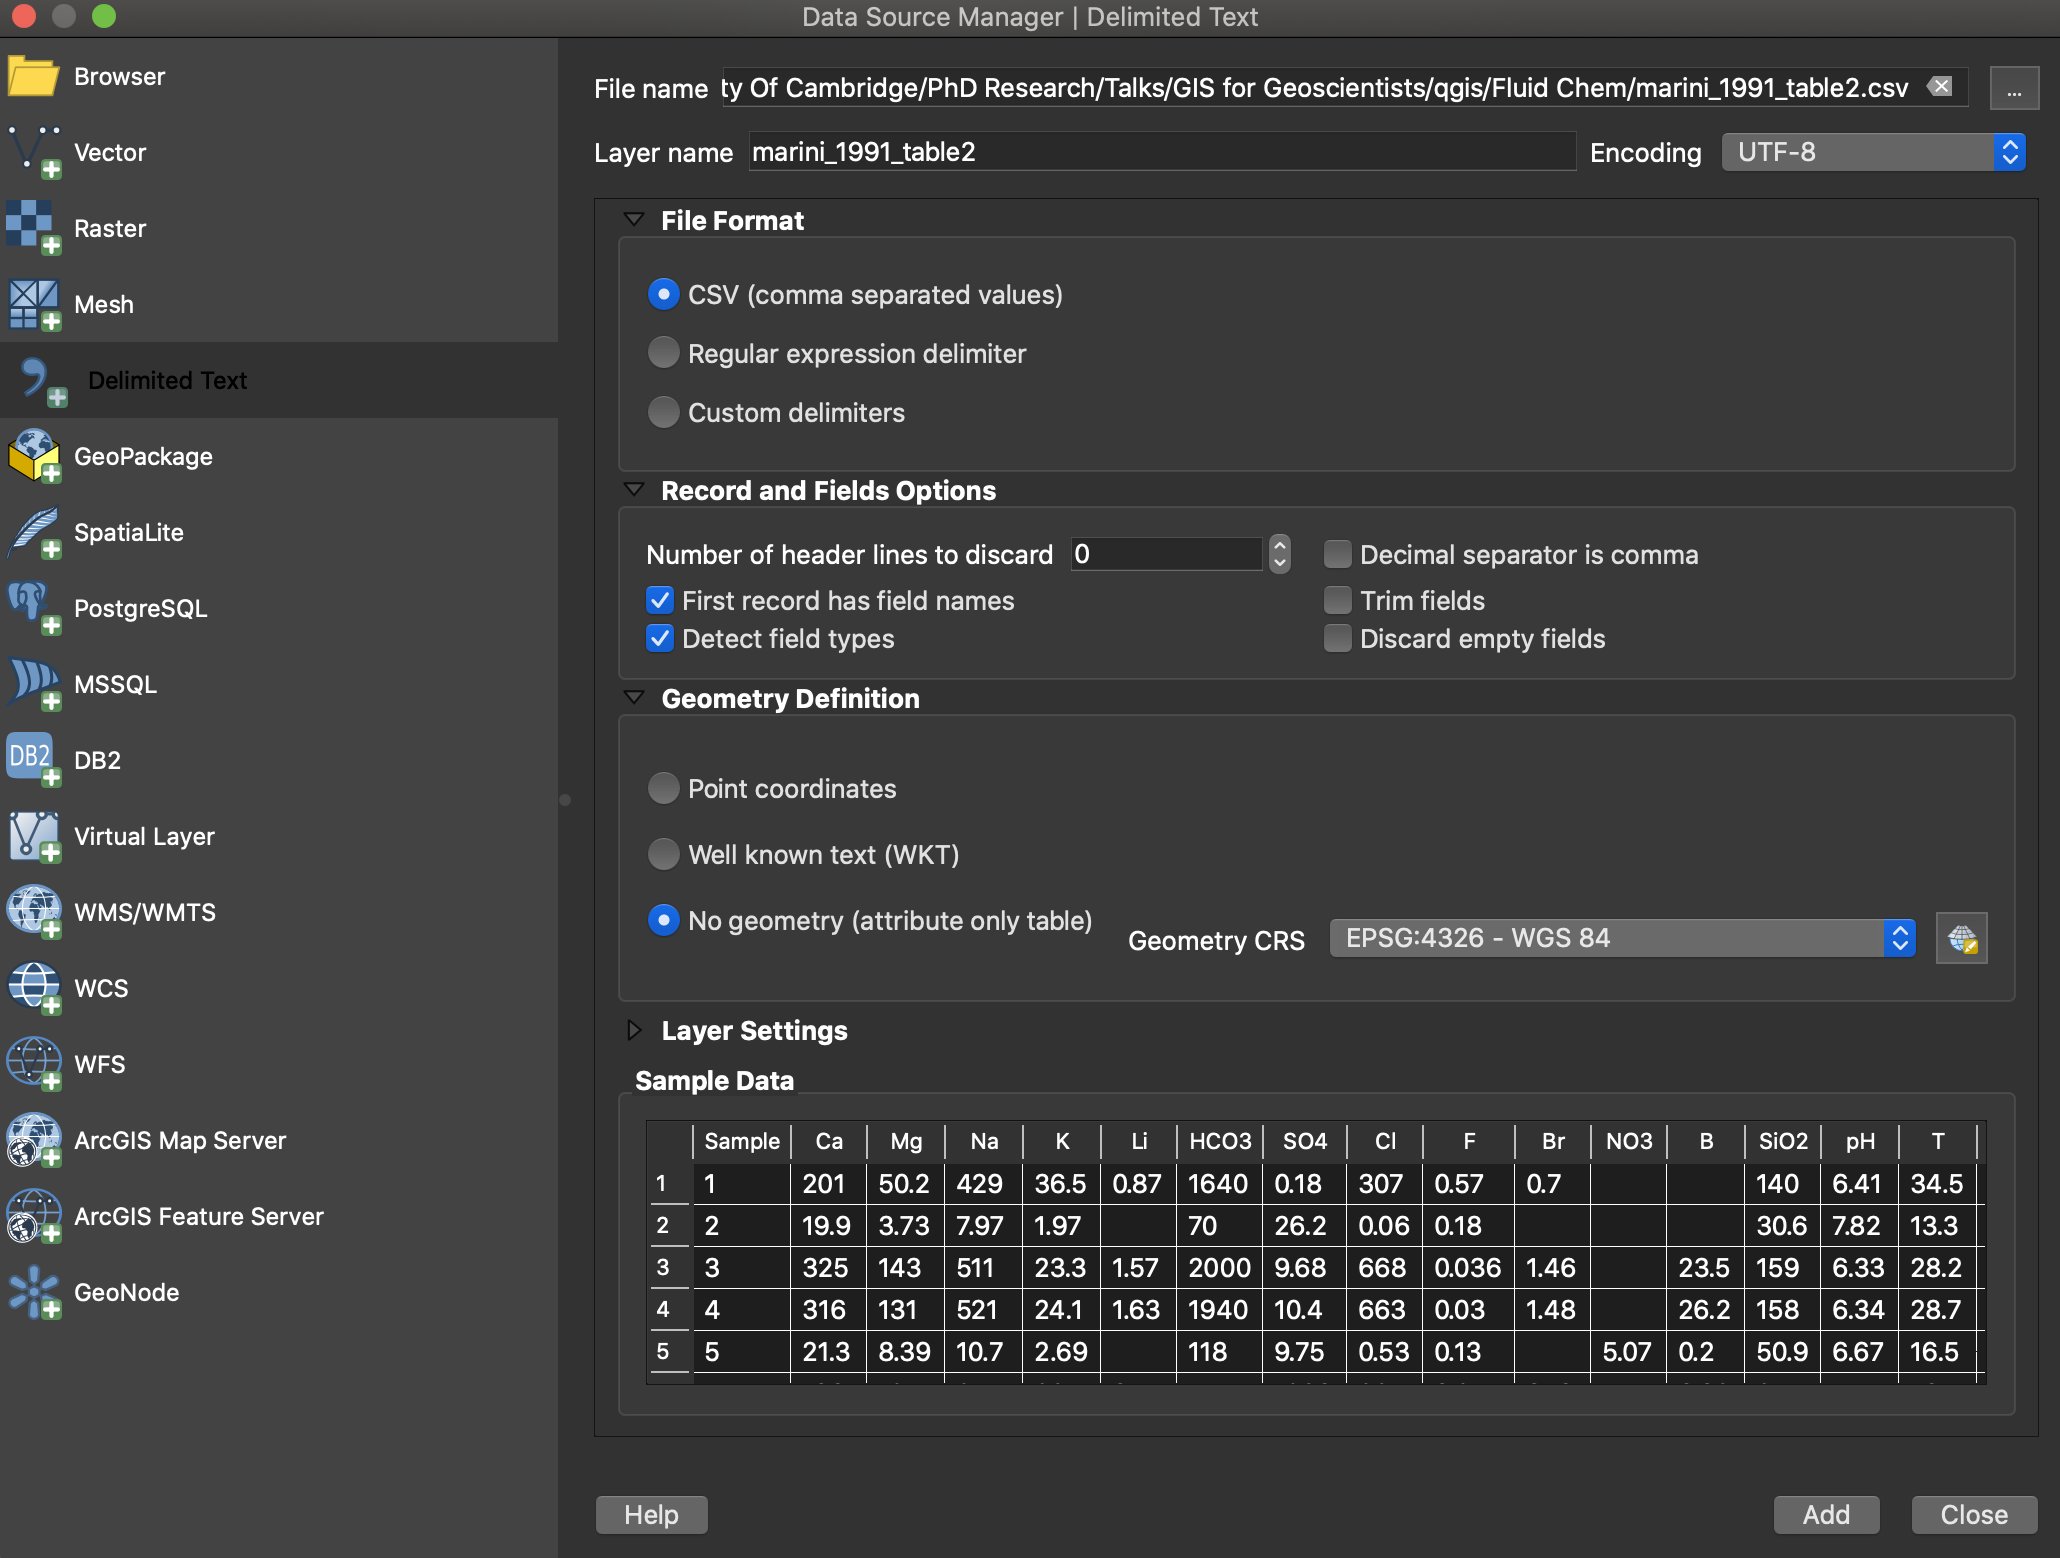
\includegraphics[width=\textwidth]{Fig_13_CSV_example.png}
    \label{fig13}
    \caption{Delimited text file import menu. Tables of CSV, TXT, Tab-separated, and most other spreadsheet formats can be read into QGIS and have a spatial dimension given to them using this menu. Details of menu options explained in text.}
\end{figure}

The final box asks you to define the geometry of the text file. What you select here is going to be very file dependent - we will deal with two different variants of text file throughout these exercises. The first one we will encounter will use the "Point Coordinates," option. Selecting this allows you to specify fields from the text file that define the latitude (Y field) and longitude (X field) of the data. This even allows you to specify a Z field (if you have elevation information). You then select a \textbf{coordinate reference system} (CRS) that these Lat/Long points are taken in relation to. \textbf{If you don't know what CRS your data is based on, it's always safe to select EPSG 4326 - WGS 84.} This will be discussed in more detail in the next section.  The second geometry option we will use is the "No Geometry," option. This is very common with older data, where an author will produce a table with sample site labels and chemical measurements, forgetting to manually record the latitude/longitude coordinates of the different sample sites.  We will use a table taken from a study on the hydrogeochemistry of Guagua Pichincha to illustrate how this data can still be given a spatial scope. The final Geometry definition option is the Well Known Text (WKT): a table format that may commonly come out of supporting geospatial libraries like GeoPandas for python. These tables will have specific "geometry," fields, and b selecting WKT you need to point QGIS to the geometry column AND say what kind of geometry this represents. We won;t work with WKT here, but it's important to know what WKT is. 

\begin{figure}[htbp]
    \centering
    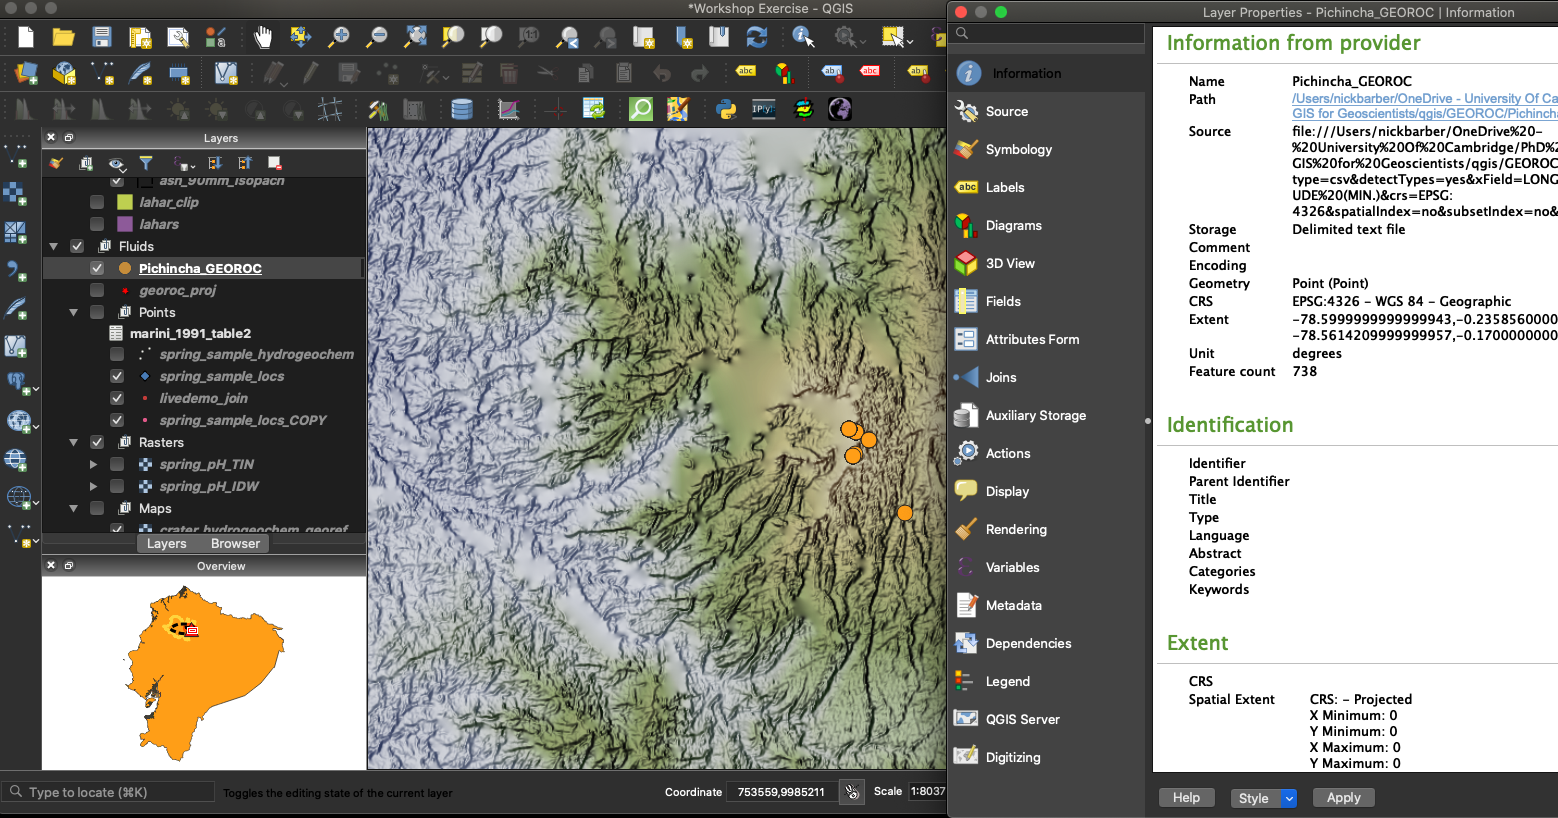
\includegraphics[width=0.9\textwidth]{Fig_14_imported_csv.png}
    \label{fig13}
    \caption{View of QGIS Project after importing a text file called "Pichincha\-GEOROC. Right clicking on this layer, selecting Properties, and navigating to the "Information" table let's us see that despite appearing like a Vector file on the map canvas, the data is still stored as a text file. We need to convert this data to a different format to interact with it in a meaningful way.}
\end{figure}

Right clicking on your imported text file and selecting "Properties" allows you to inspect the relevant features of your newly imported text file (Figure 14). If you follow the "Point Coordinates," Geometry option, you may be confused to find that, despite the points in your file plotting on your map canvas (orange circles in Figure 14), you can't interact as you would with a normal shapefile. For example, you can't edit the existing points, or add new points. The reason for this is because \textbf{an imported Point Coordinate text file, despite looking like vector data, is imported as a text file layer without additional processing}. This data format has very limited applicability in common geospatial operations, and many new users will be stumped as to why their newly imported data isn't working as intended. The solution to this issue involves an operation we will use a lot in these exercises: the \textbf{"Export Layer as.."} dialogue. 

\begin{figure}[htbp]
    \centering
    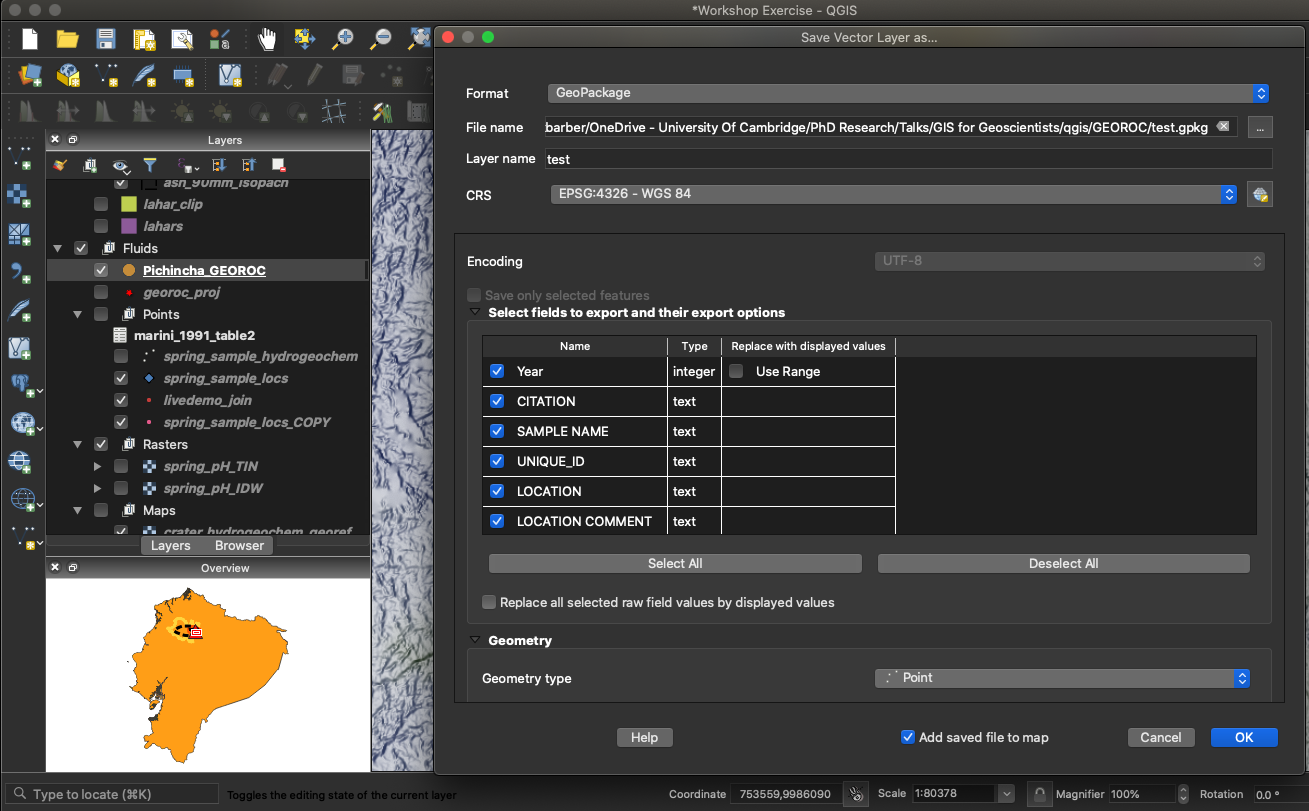
\includegraphics[width=0.9\textwidth]{Fig_15_saving_csv.png}
    \label{fig13}
    \caption{Delimited text file import menu. Tables of CSV, TXT, Tab-separated, and most other spreadsheet formats can be read into QGIS and have a spatial dimension given to them using this menu. Details of menu options explained in text.}
\end{figure}

To bring this menu up, select the text file of interest (e.g. Pichincha\_GEOROC in Figure 15) and right click on it. Scroll down to the bottom of the menu that appears, and select "Export" followed by "Save Feature As..." which brings up the menu you see in Figure 15. This menu has a lot of options, some of which we will explore in more detail later. For now, the options I want you to focus on are, first and foremost, the "Format" dropdown. There's no rule that says your imported text file, which in this case has a point geometry, needs to be in any prescribed format. The two most likely choices here are "ESRI Shapefile" and "Geopackage," following the discussion in Section 6.1. Once you select the format you'd like, click the ellipsis next to "File name," and navigate to the folder in your hard drive where you want to store the file. Select a name in this menu, and that name will be transcribed into the "Layer name" field in the "Save feature as" dialogue. Note: \textbf{Layer name(s) can ALWAYS be different from the actual file name.} This will come in handy as we seek to organize our work space. You likely won't need to the change the Encoding or Field options, but note that when saving this text file to a new vector layer, you have the option to "forget" certain attribute fields (you do this by deselecting a particular field). Finally, make sure you specify the "Geometry" in question. In this case, we know the records plot as points following the "Point Coordinate," option we choose when importing the data. Select "Ok" to make your conversion final. If you have the "Add saved file to map" option checked, your identical looking vector formatted table will instantly be added, and will tend to be plotted above the delimited text layer on the canvas. This Export process is something we will do with a number of different layers through our exercise. But at last, we are done with Data Import! Let's move on to taking some of our newly imported data, and decide what projection system to use. 

\section{Spatial Referencing}

When approaching GIS independently for this first time, the prompts that come up asking you to provide a "Datum transformation," or warning you that there is a projection issue with your data, may seem like minor kinks in an otherwise straightforward analytical routine. When being taught GIS in the classroom, projections + coordinate systems are usually discussed theoretically, but in practice, a lecturer will say "use this one," and the exercise will proceed without much greater reflection. On your own, the data you will use often has a preferred CRS and projection system, so a a similar disregard may be paid to this topic. You may yet get away with ignoring spatial referencing and projections: many global datasets can get by with simplifying assumptions, and great supporting metadata built in to GIS products may remove the need for you, the geologist, to make any new decisions. 

But these are limited exceptions to one very important general rule: \textbf{The 2D maps we use to show the location of objects on the Earth inherently distort the complex 3D geometry of the Earth.} The goal of \textbf{spatial referencing} is to allow data created relative to to one coordinate reference system to communicate with data using a different coordinate reference system or projection system. In this section, I will limit myself to discussing the thought process behind spatial referencing: specifically, the process of selecting a CRS and a Projection system. This will be very practically minded, and will simplify some of the more complex topics like the geoid, the reference ellipsoid, equipotential surfaces, geodetic levelling, and other fascinating but challenging topics.  For a more detailed treatment of this subject's theoretical foundation, I highly recommend Chapter 4 of Huisman and de By's freely-available \textit{Principles of Geographic Information Systems.} The PDF for this textbook can be found on the course web page, under "resources." 

\subsection{Defining Coordinate Systems and Projections}

\textbf{Having already decided what the scope of our GIS project is, our priority is spatially referencing all of our data using a common, locally accurate reference system.} Keep in mind that our research question concerns a regional study of Guagua Pichincha and the surrounding Quito metropolitan area in Ecuador, South America. Following the official QGIS User guide (\url{https://docs.qgis.org/3.10/en/docs/user_manual/working_with_projections/working_with_projections.html}), a CRS is, "...a method of associating numerical coordinates with a position on the surface of the Earth." These numerical coordinates can be latitude and longitude (measured in degrees), as in our CSV import example (Section 6.3), X \& Y, or Easting and Northing (both X/Y and E/N usually measured in meters). The surface of the Earth in this case is given by a reference system, or a \textbf{datum.} 

There are several major datum's, but thanks to global cooperation following the advent of the global positioning system (GPS) in the mid 1980's, these datum's are all almost universally interchangeable. Where we are working in the Western Hemisphere, the US-designed GRS80/WGS84 is the most common. Increasingly, this datum dominates more global geospatial applications, but alternative datum's are completely valid and are widely used in regions like Europe (e.g. ETRS89). QGIS handles datum's using the PROJ projection library, which is a workhorse open source reference of thousands of existing CRS' (see \url{https://proj.org}). Reference systems are called using shorthand codes, defined by the European Petroleum Search Groups (EPSG) standard practices. For example, the WGS84 global lat/long CRS uses to EPSG code "EPSG:4326." In the various CRS dialogues in QGIS, this code is the main label used to organize CRS'. 

Thankfully, given the fact that so many datum's are interchangeable, we can select GRS80 is our baseline, and move on to the much more Given our very local focus on the area in and around Guagua Pichincha, ideally we would pick an Ecuadorian CRS. Specifically, we need a CRS that is built for regional scale analysis. Note that in this context, "regional," means at a municipal or province scale in the country of Ecuador. This semantic preference is in contrast to a "local" scale CRS, which would mean confined to one small section of G.P. (e.g. a particular drainage basin), or "national," which would encompass the whole country. Now, in practice, CRS' can be designed to encompass all three of these scales.  But defining this need, alongside our original research question and goal, will help us in picking a CRS. To do so, we can look to several resources (1) past GIS studies in the region; these are probably your best bet, as they will be based on local knowledge and the expertise of trained Ecuadorian GIS professionals, or (2) the website \url{http://www.epsg-registry.org}. This latter is where I went to find a CRS for our project, as I couldn't find much on the few Ecuadorian geological studies I consulted (note: my ability to interact with Ecuadorian geological literature is limited by my lack of fluency in Spanish; a Spanish-fluent GIS user would likely be able to get everything they need off of relevant Ecuadorian websites). Searching for Ecuador, and inspecting the vast array of CRS' that appear, I decided to use \textbf{SIRGAS 2000/UTM Zone 17S}. My reasoning for this selection follows a few lines of logic. outlined below. However, I want to emphasize that \textbf{there is no wrong CRS choice, so long as we document the CRS and acknowledge its limitations and errors:}

\begin{itemize}
    \item Following the EPSG repository query, I googled what a common CRS for work in Quito Ecuador would be. Several different GIS websites, including a companion EPSG site like \url{https://epsg.io/?q=Ecuador} emphasize how widespread SIRGAS 2000/UTM Zone 17S for Eastern South America. 
    \item Checking both the EPSG repository and epsg.io website show that this CRS was defined in the past 20 years, and was made following a collaborative South American wide standardization of CRS'. This provides a guarantee that the CRS has high quality and reliability. If you google SIRGAS 2000, you find metadata explaining that the SIRGAS initiative was a highly detailed, painstaking calibration, and resulting CRS' are highly reliable
    \item I know from previous GIS experience that UTM-oriented CRS' are excellent. UTM stands for "Universal Transverse Mercator," and UTM coordinates are used in one of the most widely applied projection systems across the world. The fact that SIRGAS 2000 is rooted to this localized, Ecuador focused slice of UTM (Zone 17S) means that local data integrity in and around Quito is excellent. 
    \item The measured accuracy of SIRGAS is 1.0m - this is good for a CRS, and means we won't have to worry about errors coming from our CRS choice too much (see Error Propagation section for more details). See: \url{https://epsg.io/31977}
\end{itemize}

With that choice made, we need to amke sure our project is set up for success. 

\subsection{Reprojection}

Now that we have discussed the projection system we are going to use in this project, we need to bring our data up to speed!

To make the Datu transform work, you have to add this line of PROJ commands to your CRS "Transformations" options: 

\begin{lstlisting}[language=bash]
    +proj=pipeline +step +proj=unitcon vert +xy_in=deg +xy_out=rad +step +proj=utm +zone=17 +south +ellps=GRS80
\end{lstlisting}

\section{Setting Up Workspace}

\section{Georeferencing Our Base Map}

\section{Creating New Features}

\section{Accounting for errors}

\section{Analysis}

\subsection{Field Calculator}

\subsection{Geoprocessing}

\subsection{Statistics Viewer}

\section{Symbology}

\subsection{Vector}

\subsection{Digital Elevation Models (DEMs)}

\subsection{3D View}

\section{Creating a Map: Layout Manager}

\section{Final Thoughts}

\section{Data Sources and Further Reading}

\section{Acknowledgements}

\newpage
\printbibliography

\end{document}
